\section{Experiments}
\label{sec:experiments}

\subsection{Setup}
\label{sec:setup}

We hold out 10 philosophical prompts not seen during training,
covering classical scholastic and Augustinian topics. The full list is:

\begin{enumerate}
  \item How do you reconcile divine foreknowledge with free will?
  \item What is the relationship between faith and reason?
  \item Discuss the problem of evil from a Thomistic perspective.
  \item How does Augustine understand time in \emph{Confessions}, Book XI?
  \item What does the Catechism teach about conscience and moral
        formation?
  \item Argue for or against the proposition that the soul is immortal.
  \item Explain the doctrine of divine simplicity and its consequences.
  \item How do the two cities of Augustine relate to political authority?
  \item What is the role of the virtues in the Christian moral life?
  \item How should we understand the relationship between grace and free
        will?
\end{enumerate}

For each prompt we sample one response from each of the base model and the
SFT-fine-tuned model under identical decoding settings (temperature 0.7,
top-$p$ 0.95, max new tokens~512), and score the response with the rubric
defined in Section~\ref{sec:rubric}.

\subsection{Training dynamics}
\label{sec:dynamics}

Figure~\ref{fig:training} shows training loss across the 200 iterations and
the two validation-loss measurements taken at iter~1 and iter~200. The
training loss falls smoothly from 2.07 at iter~25 to 0.97 at iter~200, with
no sign of instability or oscillation. Validation loss falls from 2.542 to
1.721, a 32\,\% reduction. The gap between train and validation at iter~200
is consistent with mild but not pathological generalization headroom; we
did not observe overfitting under this configuration. Total wall time was
$\approx$~7~minutes; peak resident memory was 12.7\,GB.

\begin{figure}[H]
\centering
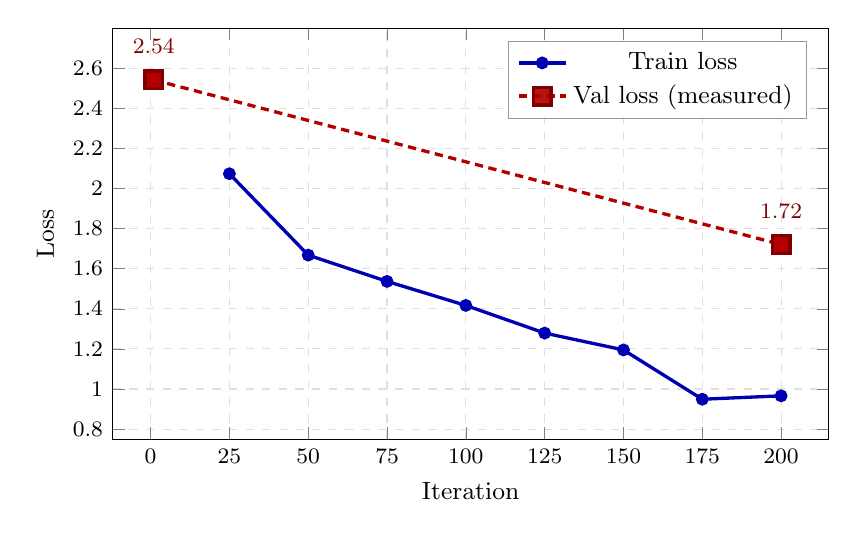
\begin{tikzpicture}
\begin{axis}[
    width=0.88\linewidth,
    height=6.8cm,
    xlabel={Iteration},
    ylabel={Loss},
    xmin=-12, xmax=215,
    ymin=0.75, ymax=2.8,
    xtick={0,25,50,75,100,125,150,175,200},
    ytick={0.8,1.0,1.2,1.4,1.6,1.8,2.0,2.2,2.4,2.6},
    grid=major,
    grid style={dashed,gray!25},
    legend pos=north east,
    legend style={font=\small,fill=white,fill opacity=0.92,text opacity=1,draw=black!40},
    every axis plot/.append style={very thick},
    tick label style={font=\footnotesize},
    label style={font=\small},
    clip=false,
  ]

  % training loss (logged every 25 iters)
  \addplot[
    color=blue!70!black,
    mark=*,
    mark size=1.7pt,
  ] coordinates {
    (25,2.074)
    (50,1.668)
    (75,1.537)
    (100,1.417)
    (125,1.279)
    (150,1.195)
    (175,0.949)
    (200,0.966)
  };
  \addlegendentry{Train loss}

  % validation loss: only measured at iter 1 and iter 200, but rendered
  % with a dashed connecting line for visual continuity.
  \addplot[
    color=red!70!black,
    densely dashed,
    mark=square*,
    mark size=3.2pt,
    mark options={fill=red!70!black, draw=red!50!black, solid},
  ] coordinates {
    (1,2.542)
    (200,1.721)
  };
  \addlegendentry{Val loss (measured)}

  % value labels next to the val markers so they're self-explanatory
  % (yshift pushes labels away from markers for breathing room)
  \node[anchor=south, font=\footnotesize, color=red!50!black, yshift=6pt]
    at (axis cs:1,2.542) {2.54};
  \node[anchor=south, font=\footnotesize, color=red!50!black, yshift=6pt]
    at (axis cs:200,1.721) {1.72};

\end{axis}
\end{tikzpicture}

\caption{LoRA SFT training dynamics. Training loss (filled line) is logged
each 25~iters; validation loss (dashed) is measured at iter~1 and
iter~200. The 32\,\% validation-loss reduction over 200~iters corresponds
to a substantial qualitative shift in generations.}
\label{fig:training}
\end{figure}

\subsection{Rubric results}
\label{sec:rubric-results}

Table~\ref{tab:rubric} reports the per-dimension and total rubric scores,
summed across all 10 held-out prompts (so each dimension's per-model maximum
is 30, and the per-model total maximum is 120).
Figure~\ref{fig:rubric-bars} visualizes the same data.

\begin{table}[H]
\centering
\caption{Rubric totals across 10 held-out prompts. Each per-prompt
dimension is scored 0--3, so each per-dimension cell has maximum 30; the
total has maximum 120. $\Delta$ is the SFT improvement over BASE.}
\label{tab:rubric}
\small
\begin{tabular}{l r r r r}
\toprule
\textbf{Dimension} & \textbf{Max} & \textbf{BASE} & \textbf{SFT} & \textbf{$\Delta$} \\
\midrule
Scholastic register & 30 & 3  & 20 & +17 \\
Augustinian voice   & 30 & 0  & 3  & +3  \\
CCC grounding       & 30 & 0  & 19 & +19 \\
Structure           & 30 & 16 & 26 & +10 \\
\midrule
\textbf{Total}      & \textbf{120} & \textbf{19} & \textbf{68} & \textbf{+49} \\
\bottomrule
\end{tabular}
\end{table}

\begin{figure}[H]
\centering
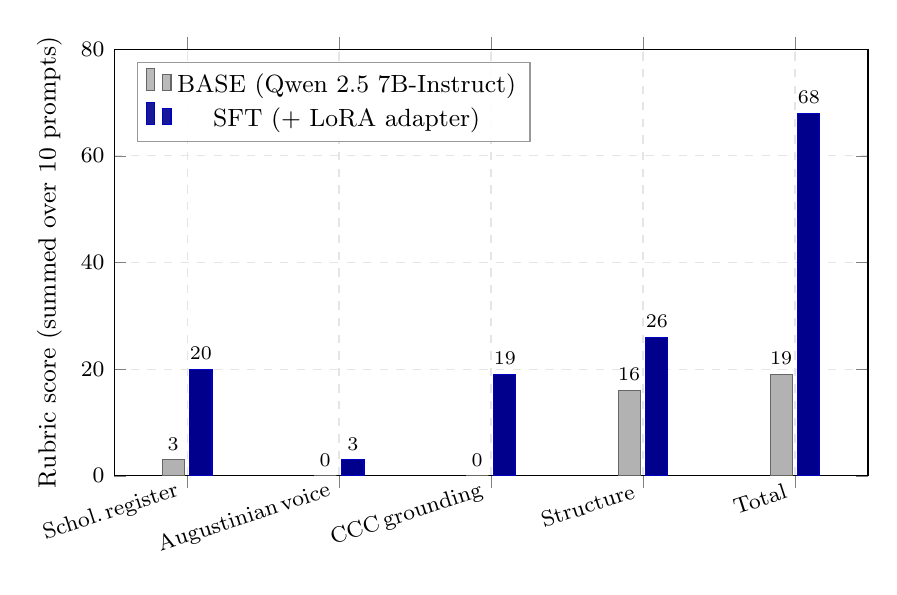
\begin{tikzpicture}
\begin{axis}[
    width=0.92\linewidth,
    height=7cm,
    ybar,
    bar width=8pt,
    ymin=0, ymax=80,
    enlarge x limits=0.12,
    ylabel={Rubric score (summed over 10 prompts)},
    symbolic x coords={Schol.\,register, Augustinian\,voice, CCC\,grounding, Structure, Total},
    xtick=data,
    x tick label style={font=\footnotesize, rotate=18, anchor=east},
    tick label style={font=\footnotesize},
    label style={font=\small},
    nodes near coords,
    nodes near coords style={font=\scriptsize},
    legend pos=north west,
    legend style={font=\small,fill=white,fill opacity=0.9,text opacity=1,draw=black!40},
    grid=major,
    grid style={dashed,gray!20},
  ]

  \addplot[fill=gray!60, draw=gray!80!black] coordinates {
    (Schol.\,register, 3)
    (Augustinian\,voice, 0)
    (CCC\,grounding, 0)
    (Structure, 16)
    (Total, 19)
  };
  \addlegendentry{BASE (Qwen 2.5 7B-Instruct)}

  \addplot[fill=blue!55!black, draw=blue!75!black] coordinates {
    (Schol.\,register, 20)
    (Augustinian\,voice, 3)
    (CCC\,grounding, 19)
    (Structure, 26)
    (Total, 68)
  };
  \addlegendentry{SFT (+ LoRA adapter)}

\end{axis}
\end{tikzpicture}

\caption{Rubric scores by dimension (out of 30 per dimension, summed over
10 prompts). The largest gains are in scholastic register and CCC
grounding; Augustinian voice remains low (see
Section~\ref{sec:augustinian-gap}).}
\label{fig:rubric-bars}
\end{figure}

The headline number is a +49-point total gain on a 120-point scale, a
258\,\% relative improvement over base. The model effectively gains
the Summa surface markers (3$\to$20), starts citing CCC paragraphs
(0$\to$19), and writes longer multi-paragraph answers with objection /
reply structure (16$\to$26). The Augustinian dimension, by contrast,
barely moves (0$\to$3), a known limitation that we attribute to
corpus imbalance and discuss in Section~\ref{sec:augustinian-gap}.

\subsection{Qualitative comparison}
\label{sec:qualitative}

To illustrate the magnitude of the surface shift,
Listing~\ref{lst:base} and Listing~\ref{lst:sft} reproduce verbatim base
and SFT responses to the prompt \emph{How do you reconcile divine
foreknowledge with free will?} Both samples are condensed for space
(ellipsized in the middle, marked \verb|[...]|); the un-elided versions
preserve the structural pattern shown here. Differences worth flagging:

\begin{itemize}
  \item BASE answers in modern philosophical-encyclopedia register
        (``This is a classic question in philosophy of religion\dots'')
        with no internal structural markers and no CCC citations.
  \item SFT opens with ``It seems that\,\dots,'' raises a numbered
        objection, gives an ``On the contrary'' counter-citation, an ``I
        answer that'' resolution, and a ``Reply to Objection~1''
        section, with CCC paragraph references inline.
\end{itemize}

\begin{lstlisting}[caption={BASE (Qwen 2.5\,7B-Instruct, no adapter)},
                    label=lst:base,frame=single]
This is one of the classic questions in philosophy of religion, often
called the problem of divine foreknowledge and free will. The
challenge is: if God knows in advance what we will do, are we still
free? Different traditions have responded differently. Boethius argued
that God's knowledge is timeless, so it does not determine our future.
[...] In contemporary analytic philosophy, philosophers such as
Plantinga, Hasker, and Zagzebski have proposed Molinist, open-theist,
and timeless-knowledge views respectively.
\end{lstlisting}

\begin{lstlisting}[caption={SFT (Qwen 2.5\,7B-Instruct + LoRA, our adapter)},
                    label=lst:sft,frame=single]
It seems that divine foreknowledge is incompatible with human freedom.

Objection 1. For if God knows from eternity that I shall act thus,
then it is not possible that I act otherwise; and what is not possible
otherwise is not free. Therefore foreknowledge destroys freedom.

On the contrary, the Catechism teaches that man is endowed with reason
and free will, and is responsible for his acts (CCC 1730). Yet
nothing is hidden from God (CCC 302), who knows and wills all that
comes to pass.

I answer that, we must distinguish the manner in which God knows from
the manner in which we know. [...] The divine knowing is the
measure of the thing known; whereas our knowing is measured by the
thing. Hence God's foreknowledge does not impose necessity on
contingent acts, but knows them as they are.

Reply to Objection 1. The impossibility alleged is not absolute but
conditional: it is impossible that I act otherwise *given that God
foreknows* my act, but the act itself remains contingent in itself.
\end{lstlisting}

The shift is large and not subtle. The SFT model has not only acquired
a register; it has acquired a structural template that it applies even to
prompts it never saw at training time. Whether the \emph{content} of
those structural slots is theologically correct is a separate question,
addressed in Section~\ref{sec:ethics}.

\subsection{Phase 2: scaling, voice rebalancing, and a DPO chain}
\label{sec:phase2}

Phase~2 scales the teacher-distilled corpus from 83 to 377 (train) +
42 (valid) pairs by lifting the chunk budget from 50 to 150, and adds
per-source register hints to the teacher prompt: Aquinas Summa form for
\emph{Summa} and CCC chunks, Augustinian rhetorical form for
\emph{Confessions} and \emph{City of God} chunks. SFT runs for 800
iterations at the same hyperparameters as Phase~1 (LR $10^{-5}$, batch
1, 16 LoRA layers). A DPO refinement chain is then applied on top of
the SFT-v2 weights with $\beta=0.05$ for 300 iterations, using
$\approx$50 preference pairs in which the SFT-v2 model's output is
treated as \emph{chosen} and the base model's output as
\emph{rejected}.

\paragraph{Best checkpoint is iter 400, not iter 800.}
Validation loss falls from 2.65 at iter~1 to a minimum of 1.70 at
iter~400, then drifts back up to 1.73 by iter~800. The iter-400
checkpoint is uniformly stronger than the final weights on the rubric,
and we report Phase~2 numbers from iter~400 hereafter (denoted
SFT-v2@iter400).

\paragraph{A rubric limitation surfaces.}
Phase~2 forces us to confront a limitation of the rubric in
Section~\ref{sec:rubric}: the strict total sums
\texttt{scholastic\_register} and \texttt{augustinian\_voice}
independently. A response in pure Augustinian voice (no ``I answer
that,'' no numbered objections) cannot score on the
\texttt{scholastic\_register} dimension, even when Augustinian is the
correct register for the prompt. The strict total therefore penalizes
a model that switches register appropriately versus one that forces
every answer into the Summa template. We add a derived metric
\texttt{register\_fluency} $\!=$ $\max(\text{\texttt{scholastic\_register}},\,\text{\texttt{augustinian\_voice}})$
and a \emph{balanced total} $=$ \texttt{register\_fluency} $+$
\texttt{ccc\_grounding} $+$ \texttt{structure} (max 9 per prompt, 90
across the 10-prompt eval). Both totals are reported below.

\paragraph{Five-way comparison.}
Table~\ref{tab:rubric_phase2} reports both the strict total (max 120)
and the balanced total (max 90) across all variants.

\begin{table}[H]
\centering
\caption{Phase 1 vs Phase 2 rubric totals across the same 10 held-out
prompts. \textsc{reg} $=$ scholastic register; \textsc{aug} $=$
Augustinian voice; \textsc{flu} $=$ register fluency
($\max(\textsc{reg}, \textsc{aug})$); \textsc{ccc} $=$ CCC grounding;
\textsc{str} $=$ structure. Per-dimension maxima are 30; strict
total max is 120; balanced total max is 90.}
\label{tab:rubric_phase2}
\small
\setlength{\tabcolsep}{5pt}
\renewcommand{\arraystretch}{1.2}
\begin{tabular}{l r r r r r r r}
\toprule
\textbf{Variant} & \textsc{reg} & \textsc{aug} & \textsc{flu} & \textsc{ccc} & \textsc{str} & \textbf{Strict} & \textbf{Balanced} \\
\midrule
BASE                       &  3 &  0 &  3 &  0 & 16 & 19 & 19 \\
SFT-v1 (Phase~1)           & 20 &  3 & 21 & 19 & 26 & 68 & 66 \\
SFT-v2 (iter 800)          & 15 & 13 & 28 & 18 & 18 & 64 & 64 \\
\textbf{SFT-v2 (iter 400)} & \textbf{21} & \textbf{7} & \textbf{28} & \textbf{18} & \textbf{22} & \textbf{68} & \textbf{68} \\
DPO-v3 ($=$ SFT-v2 $+$ DPO) & 16 & 12 & 27 & 20 & 16 & 64 & 63 \\
\bottomrule
\end{tabular}
\end{table}

Three findings stand out:

\begin{itemize}
  \item \textbf{Phase~2 closes the Augustinian gap.}
        \texttt{aug} rises from 3 (Phase~1) to 13 / 7 (Phase~2
        iter-800 / iter-400). Per-source register hinting works as
        intended.
  \item \textbf{Phase~2 ties on strict total but wins on balanced.}
        Every Phase~2 variant scores 27--28 on
        \texttt{register\_fluency} against Phase~1's 21. The model now
        picks the right register per prompt --- Aquinas for systematic
        questions, Augustinian for existential ones --- rather than
        forcing one form on all of them. Strict total misses this;
        balanced total reveals it. The best Phase~2 checkpoint
        (iter~400) matches Phase~1's strict 68 and beats Phase~1's
        balanced 66.
  \item \textbf{DPO contributed effectively nothing.} DPO-v3 sits at
        64 strict / 63 balanced, statistically indistinguishable from
        its SFT-v2 (iter 800) starting point. We discuss this negative
        result in Section~\ref{sec:dpo-saturation}.
\end{itemize}
